\documentclass[fleqn,11pt]{article}

\usepackage[letterpaper,margin=0.75in]{geometry}

\usepackage{amsmath}
\usepackage{booktabs}
\usepackage{graphicx}
\usepackage{listings}

\setlength{\parindent}{1.4em}

\begin{document}

\lstset{
  language=Python,
  basicstyle=\small,          % print whole listing small
  keywordstyle=\bfseries,
  identifierstyle=,           % nothing happens
  commentstyle=,              % white comments
  stringstyle=\ttfamily,      % typewriter type for strings
  showstringspaces=false,     % no special string spaces
  numbers=left,
  numberstyle=\tiny,
  numbersep=5pt,
  frame=tb,
}

\title{Network Simulation (Lab 1) Report}

\author{Luke Dickinson}

\date{1/25/2017}

\maketitle

\section{Introduction}

In order to measure the way a basic network performs, we used a network simulator called Bene to simulate a number of different situations. In each of these situations, we will show how the simulation is set up, what the simulation resulted to, and alternate calculations to show that the result from the simulation is correct.
\subsubsection{Terms and Abbreviations }

In order to increase readability, abbreviations will be used throughout the paper. The following terms may be use in the abbreviated form:
\begin{align*}
Packet &= p\\
Node &= n\\
CreationTime &= cTime\\
ProcessingDelay &= procDelay\\
PropagationDelay &= propDelay\\
TransmissionDelay &= tDelay\\
QueueingDelay &= qDelay\\
\end{align*}

\section{Two Nodes}
This section includes a network that consisting of 2 nodes. The setup required for the simulations in this section is the same for each case. To setup the simulation, we first reset the scheduler for the simulation. Next, we set up the network by create a Network object by passing a network configuration file (which will be described in each simulation). After that, we set up the route information between the nodes. Finally, we setup a handler to print out information about packets received at node$_2$. The following code snippet performs the setup:
\begin{lstlisting}
# parameters
Sim.scheduler.reset()

# setup network
net = Network('lab1-onehopX.txt')

# setup routes
n1 = net.get_node('n1')
n2 = net.get_node('n2')
n1.add_forwarding_entry(address=n2.get_address('n1'), link=n1.links[0])
n2.add_forwarding_entry(address=n1.get_address('n2'), link=n2.links[0])

# setup app
d = DelayHandler()
net.nodes['n2'].add_protocol(protocol="delay", handler=d)
\end{lstlisting}

 \subsection{First simulation of a two node network}
\subsubsection{Simulation configuration}
For our first simulation of a two node network, we set the bandwidth between the nodes to 1 Mbps, and set the propagation delay between the nodes to 1 second. We send a single packet of size 1000 bytes from one node to the other at time set to 0 seconds. To do this we use the following configuration file:

\begin{lstlisting}
# n1 -- n2
n1 n2
n2 n1

# link configuration
n1 n2 1Mbps 1000ms
n2 n1 1Mbps 1000ms
\end{lstlisting}

This configuration file above is called 'lab1-onehopA.txt.' This is to be inserted into our Network constructor refered to above.
Once the network is set up, we will send our single packet to node$_2$ and then run the simulation. This is shown in the following code snippet:    

\begin{lstlisting}
#send packet(s)
p = Packet(destination_address=n2.get_address('n1'), \\
	ident=1, protocol='delay', length=1000)
Sim.scheduler.add(delay=0, event=p, handler=n1.send_packet)

# run the simulation
Sim.scheduler.run()
\end{lstlisting}

\subsubsection{Output of the simulation}
\begin{lstlisting}
(1.008, 1, 0, 1.008, 0.008, 1.0, 0)
\end{lstlisting}
This output shows that the first packet was created at 0 seconds, its identifier was 1, and the time it was received by node$_2$ was at 1.008 seconds.

\subsubsection{Verifying calculations}

We are able to calculate the time our packet is received at node$_2$ by adding the creation time of the packet, the processing delay, propagation delay, transmission delay, and queueing delay for this packet. In our simulation we are assuming that processing delay is 0. In situations of only a single packet, there is no queueing delay.

\begin{align*}
cTime_{p1} &= 0\,seconds\\
procDelay &= 0\,seconds\\
propDelay_{n1} &= 1\,second\\
tDelay_{p1\,at\,n1} &=  \frac{size\,of\,the\,packet} {link\,rates}\\
&= \frac{1000\,bytes} {1\,Mbps}\\
&=  \frac{8000\,bits} {1\,Mbps}\\
&= 0.008\,seconds\\
qDelay_{p1\,at\,n1} &= 0\,seconds\\
\\
Time\,Packet_{1}\,Is\,Received\,At\,Node_{2} &= \,cTime_{p1} + procDelay + propDelay_{n1} +\\
&\,\,\,\,\,\,\,\, + tDelay_{p1\,at\,n1} + qDelay_{p1\,at\,n1} \\
&= 0 + 0 + 1 + 0.008 + 0 \\
&= 1.008
\end{align*}

From our calculations we see that packet$_1$ is received at node$_2$ at 1.008 seconds, which matches our simulation.

 \subsection{Second simulation of a two node network}
\subsubsection{Simulation configuration}
For our second simulation of a two node network, we set the bandwidth between the nodes to 100 bps, and set the propagation delay between the nodes to 10 milliseconds. We send a single packet of size 1000 bytes from one node to the other at time set to 0 seconds. To do this, we use the following configuration file:

\begin{lstlisting}
# n1 -- n2
#
n1 n2
n2 n1

# link configuration
n1 n2 100bps 10ms
n2 n1 100bps 10ms

\end{lstlisting}

This configuration file above is called 'lab1-onehopB.txt.' This is to be inserted into our Network constructor refered to above.
Once the network is set up, we will send our single packet to node$_2$ and then run the simulation. This is shown in the following code snippet:    

\begin{lstlisting}
#send packet(s)
p = Packet(destination_address=n2.get_address('n1'), \\
	ident=1, protocol='delay', length=1000)
Sim.scheduler.add(delay=0, event=p, handler=n1.send_packet)

# run the simulation
Sim.scheduler.run()
\end{lstlisting}

\subsubsection{Output of the simulation}
\begin{lstlisting}
(80.01, 1, 0, 80.01, 80.0, 0.01, 0)
\end{lstlisting}
This output shows that the first packet was created at 0 seconds, its identifier was 1, and the time it was received by node$_2$ was at 80.01 seconds.

\subsubsection{Verifying calculations}

We are able to calculate the time our packet is received at node$_2$ by adding the creation time of the packet, the processing delay, propagation delay, transmission delay, and queueing delay for this packet. In our simulation we are assuming that processing delay is 0. In situations of only a single packet, there is no queueing delay.

\begin{align*}
cTime_{p1} &= 0\,seconds\\
procDelay &= 0\,seconds\\
propDelay_{n1} &=10\,milliseconds\\
tDelay_{p1\,at\,n1} &=  \frac{size\,of\,the\,packet} {link\,rates}\\
&= \frac{1000\,bytes}{100\,bps}\\
&=  \frac{8000\,bits}{100\,bps}\\
&= 80\,seconds\\
qDelay_{p1\,at\,n1} &= 0\,seconds\\
\\
Time\,Packet_{1}\,Is\,Received\,At\,Node_{2} &= \,cTime_{p1} + procDelay + propDelay_{n1} +\\
&\,\,\,\,\,\,\,\, + tDelay_{p1\,at\,n1} + qDelay_{p1\,at\,n1} \\
&= 0 + 0 + 0.01 + 80 + 0 \\
&= 80.01 
\end{align*}

From our calculations we see that packet$_1$ is received at node$_2$ at 80.01 seconds, which matches our simulation.

 \subsection{Third simulation of a two node network}
\subsubsection{Simulation configuration}
For our third simulation of a two node network, we set the bandwidth between the nodes to 1 Mbps, and set the propagation delay between the nodes to 10 milliseconds. We send 3 packets of size 1000 bytes from one node to the other at time set to 0 seconds. Then we send a single packet of size 1000 bytes from one node to the other at time set to 2 seconds. To do this we use the following configuration file:

\begin{lstlisting}
# n1 -- n2
#
n1 n2
n2 n1

# link configuration
n1 n2 1Mbps 10ms
n2 n1 1Mbps 10ms

\end{lstlisting}

This configuration file above is called 'lab1-onehopC.txt.' This is to be inserted into our Network constructor refered to above.
Once the network is set up, we will send our packets to node$_2$ and then run the simulation. This is shown in the following code snippet:    

\begin{lstlisting}
#send packet(s)
p = Packet(destination_address=n2.get_address('n1'), \\
	ident=1, protocol='delay', length=1000)
Sim.scheduler.add(delay=0, event=p, handler=n1.send_packet)

p2 = Packet(destination_address=n2.get_address('n1'), \\
	ident=2, protocol='delay', length=1000)
Sim.scheduler.add(delay=0, event=p2, handler=n1.send_packet)

p3 = Packet(destination_address=n2.get_address('n1'), \\
	ident=3, protocol='delay', length=1000)
Sim.scheduler.add(delay=0, event=p3, handler=n1.send_packet)

p4 = Packet(destination_address=n2.get_address('n1'), \\
	ident=4, protocol='delay', length=1000)
Sim.scheduler.add(delay=2, event=p4, handler=n1.send_packet)    

# run the simulation
Sim.scheduler.run()
\end{lstlisting}

\subsubsection{Output of the simulation}
\begin{lstlisting}
(0.018000000000000002, 1, 0, 0.018000000000000002, 0.008, 0.01, 0)
(0.026000000000000002, 2, 0, 0.026000000000000002, 0.008, 0.01, 0.008)
(0.034, 3, 0, 0.034, 0.008, 0.01, 0.016)
(2.018, 4, 2.0, 0.017999999999999794, 0.008, 0.01, 0.0)

\end{lstlisting}
This output shows that the first packet was created at 0 seconds, its identifier was 1, and the time it was received by node$_2$ was at 0.018 seconds. The second packet was created at 0 seconds, its identifier was 2, and the time it was received by node$_2$ was at 0.0260 seconds. The third packet was created at 0 seconds, its identifier was 3, and the time it was received by node$_2$ was at 0.340 seconds. The fourth packet was created at 2 seconds, its identifier was 4, and the time it was received by node$_2$ was at 2.018 seconds.

\subsubsection{Verifying calculations}
We are able to calculate the time each of our packets are received at node$_2$ by adding the creation time of the packet, the processing delay, propagation delay, transmission delay, and queueing delay for a packet. In our simulation we are assuming that processing delay is 0. 

\paragraph{Calculating the time packet$_1$ is received at node$_2$ }
\begin{align*}
cTime_{p1} &= 0\,seconds\\
procDelay &= 0\,seconds\\
propDelay_{n1} &= 10\,milliseconds\\
tDelay_{p1\,at\,n1} &=  \frac{size\,of\,the\,packet} {link\,rates}\\
&= \frac{1000\,bytes} {1\,Mbps}\\
&=  \frac{8000\,bits} {1\,Mbps}\\
&= 0.008 \,seconds\\
qDelay_{pX\,at\,nY} &= k_{X}*(tDelay_{pX\,at\,nY} - tDelay_{packetX\,at\,n(Y-1)}) \\
&\text{where k$_X$ = the number of packets at node$_y$ when packet$_x$ arrives}\\
\\
k_{1} &= 0\\
&\text{Packet$_1$ is the first packet and will not enter a queue, so k$_1$ = 0} \\
qDelay_{p1\,at\,n1} &= k_{1}*(tDelay_{p1\,at\,n1} - tDelay_{p1\,at\,n(1-1)})\\
&= (0) (0.008 - 0) \\
&= 0 \\
\\
time\,packet_{1}\,is\,received\,at\,node_{2} &= \,cTime_{p1} + procDelay + propDelay_{n\,1} +\\
&\,\,\,\,\,\,\,\, + tDelay_{p\,1\,at\,n\,1} + qDelay_{p\,1\,at\,n\,1} \\
&= 0 + 0 + 0.01 + 0.008 + 0 \\
&= 0.018\\
\text{From our calculations we see that }
&\text{packet$_1$ is received at node$_2$ at 0.018 seconds,} \\
\text{which matches our simulation.}
\end{align*}

\paragraph{Calculating the time packet$_2$ is received at node$_2$ }
\begin{align*}
cTime_{p2} &= 0\,seconds\\
procDelay &= 0\,seconds\\
propDelay_{n1} &= 10\,milliseconds\\
&\text{As packet 1 and 2, are the same size, the value for}\\
&\text{tDelay$_{p1\,at\,n1}$ is the same as tDelay${_p2\,at\,n1}$}\\
&\text{So,}\\
tDelay_{p2\,at\,n1} &=  0.008 \,seconds\\
qDelay_{pX\,at\,nY} &= k_{X}*(tDelay_{pX\,at\,nY} - tDelay_{packetX\,at\,n(Y-1)}) \\
&\text{where k$_X$ = the number of packets at node$_y$ when packet$_x$ arrives}\\
\\
k_{2} &= 1\\
&\text{Packets 1, 2, and 3 arrive at node$_1$ at 0 seconds.}\\
&\text{When these are the these packets created,}\\
&\text{there are no other packets at node$_1$.}\\
&\text{As packet$_1$ is the only packet in front of packet$_2$, k$_2$ = 1.} \\
qDelay_{p2\,at\,n1} &= k_{2}*(tDelay_{p2\,at\,n1} - tDelay_{p2\,at\,n(1-1)})\\
&= (1) (0.008 - 0) \\
&= 0.008 \\
\\
time\,packet_{2}\,is\,received\,at\,node_{2} &= \,cTime_{p2} + procDelay + propDelay_{n\,1} +\\
&\,\,\,\,\,\,\,\, + tDelay_{p\,2\,at\,n\,1} + qDelay_{p\,2\,at\,n\,1} \\
&= 0 + 0 + 0.01 + 0.008 + 0.008 \\
&= 0.026\\
\text{From our calculations we see that }
&\text{packet$_2$ is received at node$_2$ at 0.026 seconds,} \\
\text{which matches our simulation.}
\end{align*}
\paragraph{Calculating the time packet$_3$ is received at node$_2$ }
\begin{align*}
cTime_{p3} &= 0\,seconds\\
procDelay &= 0\,seconds\\
propDelay_{n1} &= 10\,milliseconds\\
&\text{As packet 1 and 3 are the same size, the value for}\\
&\text{tDelay$_{p1\,at\,n1}$ is the same as tDelay${_p3\,at\,n1}$}\\
&\text{So,}\\
tDelay_{p3\,at\,n1} &=  0.008 \,seconds\\
qDelay_{pX\,at\,nY} &= k_{X}*(tDelay_{pX\,at\,nY} - tDelay_{packetX\,at\,n(Y-1)}) \\
&\text{where k$_X$ = the number of packets at node$_y$ when packet$_x$ arrives}\\
\\
k_{3} &= 2\\
&\text{Packets 1, 2, and 3 arrive at node$_1$ at 0 seconds.}\\
&\text{When these are the these packets created,}\\
&\text{there are no other packets at node$_1$.}\\
&\text{As packet$_1$ and packet$_2$ are the only packets in front of packet$_3$, k$_3$ = 2.} \\
qDelay_{p3\,at\,n1} &= k_{3}*(tDelay_{p3\,at\,n1} - tDelay_{p3\,at\,n(1-1)})\\
&= (2) (0.008 - 0) \\
&= 0.016 \\
\\
time\,packet_{3}\,is\,received\,at\,node_{2}  &= \,cTime_{p2} + procDelay + propDelay_{n\,1} +\\
&\,\,\,\,\,\,\,\, + tDelay_{p\,2\,at\,n\,1} + qDelay_{p\,2\,at\,n\,1} \\
&= 0 + 0 + 0.01 + 0.008 + 0.016 \\
&= 0.034\\
\text{From our calculations we see that }
&\text{packet$_3$ is received at node$_2$ at 0.034 seconds,} \\
\text{which matches our simulation.}
\end{align*}
\paragraph{Calculating the time packet$_4$ is received at node$_2$ }
\begin{align*}
cTime_{p4} &= 2\,seconds\\
procDelay &= 0\,seconds\\
propDelay_{n1} &= 10\,milliseconds\\
&\text{As packet 1 and 4 are the same size, the value for}\\
&\text{tDelay$_{p1\,at\,n1}$ is the same as tDelay${_p4\,at\,n1}$}\\
&\text{So,}\\
tDelay_{p4\,at\,n1} &=  0.008 \,seconds\\
qDelay_{pX\,at\,nY} &= k_{X}*(tDelay_{pX\,at\,nY} - tDelay_{packetX\,at\,n(Y-1)}) \\
&\text{where k$_X$ = the number of packets at node$_y$ when packet$_x$ arrives}\\
\\
k_{3} &= 2\\
&\text{Packet$_ 4$ arrives at node$_1$ at 2 seconds.}\\
&\text{The packet previous to packet$_4$, packet$_3$, leaves node$_1$ at}\\
&\text{(packet$_3$ arrival time to node$_2$) - (propDelay$_{n1}$) =}\\
&\text{0.034 - 0.01 = 0.024 seconds. }\\
&\text{Because the previous packet to packet$_4$, packet$_3$, leaves node$_1$}\\
&\text{before packet$_4$ arrives, packet$_4$ does not enter the queue. So k = 0.} \\
qDelay_{p4\,at\,n1} &= k_{4}*(tDelay_{p4\,at\,n1} - tDelay_{p4\,at\,n(1-1)})\\
&= (0) (0.008 - 0) \\
&= 0 \\
\\
time\,packet_{4}\,is\,received\,at\,node_{2}  &= \,cTime_{p2} + procDelay + propDelay_{n\,1} +\\
&\,\,\,\,\,\,\,\, + tDelay_{p\,2\,at\,n\,1} + qDelay_{p\,2\,at\,n\,1} \\
&= 2 + 0 + 0.01 + 0.008 + 0 \\
&= 2.018\\
\text{From our calculations we see that }
&\text{packet$_4$ is received at node$_2$ at 2.018 seconds,} \\
\text{which matches our simulation.}
\end{align*}
\section{Three Nodes}
This section includes a network that consisting of 3 nodes. The setup required for the simulations in this section is the same for each case. To setup the simulation, we first reset the scheduler for the simulation. Next, we set up the network by create a Network object by passing a network configuration file (which will be described in each simulation). After that, we set up the route information between the nodes. Finally, we setup a handler to print out information about packets received at node$_3$. The following code snippet performs the setup:
\begin{lstlisting}
# parameters
Sim.scheduler.reset()

# setup network
#net = Network('lab1-twohopA.txt')
net = Network('lab1-twohopA2.txt')

# setup routes
n1 = net.get_node('n1')
n2 = net.get_node('n2')
n3 = net.get_node('n3')
n1.add_forwarding_entry(address=n2.get_address('n1'), link=n1.links[0])
n1.add_forwarding_entry(address=n3.get_address('n2'), link=n1.links[0])
n2.add_forwarding_entry(address=n1.get_address('n2'), link=n2.links[0])
n2.add_forwarding_entry(address=n3.get_address('n2'), link=n2.links[1])
n3.add_forwarding_entry(address=n2.get_address('n3'), link=n3.links[0])
n3.add_forwarding_entry(address=n1.get_address('n2'), link=n3.links[0])

# setup app
d = DelayHandler()
net.nodes['n3'].add_protocol(protocol="delay", handler=d)
\end{lstlisting}
\subsection{First simulation of a three node network}
\subsubsection{Simulation configuration}
For our first simulation of a three node network, we set the bandwidth between the node1 and node2 to 1 Mbps, the bandwidth from node2 to node3 to 1 Mbps, set the propagation delay between the node1 and node2 to 100 milliseconds, and set the propagation delay between the node2 and node3 to 100 milliseconds. We send a 1000 packets, each 1000 bytes in size through the network with the source being node 1 and the destination being node 3.  to node one node to the other at time set to 0 seconds. To do this we use the following configuration file:
\begin{lstlisting}
# n1 -- n2 -- n3
n1 n2
n2 n1
n2 n3
n3 n2
# link configuration
n1 n2 1Mbps 100ms
n2 n1 1Mbps 100ms
n2 n3 1Mbps 100ms
n3 n2 1Mbps 100ms
\end{lstlisting}

Once the network is set up, we will send a single file in 1000 packets to node three and then run the simulation. In order to avoid queueing issues (like overflowing the simulated queue), we will control the time each packet is sent so that each packet will be begin its process as its previous packet leaves node 1. This is shown in the following code snippet:    

\begin{lstlisting}
trasmissionDelay = 8.0/1000.0    
# send packets
for i in range(1,1001):
    calculatedDelay = (i-1) * trasmissionDelay
    p = Packet(destination_address=n3.get_address('n2'), ident=i, protocol='delay', length=1000)
    Sim.scheduler.add(delay=calculatedDelay, event=p, handler=n1.send_packet)
# run the simulation
Sim.scheduler.run() 
\end{lstlisting}
\subsubsection{Output of the simulation}
Last 5 entries:
\begin{lstlisting}
(8.176000000000007, 996, 7.96, 0.2160000000000073, 0.016, 0.2, 6.217248937900877e-15)
(8.184000000000006, 997, 7.968, 0.2160000000000064, 0.016, 0.2, 6.217248937900877e-15)
(8.192000000000007, 998, 7.976, 0.2160000000000073, 0.016, 0.2, 6.217248937900877e-15)
(8.200000000000006, 999, 7.984, 0.2160000000000064, 0.016, 0.2, 6.217248937900877e-15)
(8.208000000000007, 1000, 7.992, 0.2160000000000073, 0.016, 0.2, 6.217248937900877e-15)
\end{lstlisting}
The entire file is transfered when the last packet arrives at node$_3$. This output shows that the last packet arrived at node$_3$ at 8.208 seconds.
\subsubsection{Verifying calculations}
We are able to calculate the time our file is received at node$_3$ by calculating the time our last packet, packet$_{1000}$, is received at node $_3$. We calculate the time it takes for packet$_{1000}$ to reach node$_2$ by adding the creation time, processing delay, propagation delay, transmission delay, and queueing delay for packet$_{1000}$ going to node$_2$. We then can calculate the total time it takes to get to node$_3$ by adding the arrival time to node$_2$ for packet$_{1000}$ to the processing delay, propagation delay, transmission delay, and queueing delay for packet$_{1000}$ going to node$_3$. In our simulation we are assuming that processing delay is 0. As we are throttling our creation time of each packet, we will have no queueing delay at node 1. Also, because all of the links in our network are the same speed, every time a packet reaches a node the previous node would have just left. Therefore, there is no queuing delay for node 2 either.

\paragraph{Calculating the time packet$_{1000}$ is received at node$_2$ }
\begin{align*}
tDelay_{p1000\,at\,n1} &=  \frac{size\,of\,the\,packet} {link\,rates}\\
&= \frac{1000\,bytes} {1\,Mbps}\\
&=  \frac{8000\,bits} {1\,Mbps}\\
&= 0.008 \,seconds\\
cTime_{p1000} &= (1000-1) *tDelay_{n1}\,seconds\\
&= (999) *(0.008)\,seconds\\
&= 7.992\,seconds\\
procDelay &= 0\,seconds\\
propDelay_{n1} &= 0.1\,seconds\\
qDelay_{p1000\,at\,n1} &= 0\\
time\,packet_{1000}\,is\,received\,at\,node_{2} &= \,cTime_{p1000} + procDelay + propDelay_{n\,1} +\\
&\,\,\,\,\,\,\,\, + tDelay_{p\,10000,at\,n\,1} + qDelay_{p\,1000\,at\,n\,1}\\
&= 7.992 + 0 + 0.1 + 0.008 + 0\,seconds\\
&= 8.1\,seconds
\end{align*}

\paragraph{Calculating the time packet$_{1000}$ is received at node$_2$ }
\begin{align*}
tDelay_{p1000\,at\,n2} &=  \frac{size\,of\,the\,packet} {link\,rates}\\
&= \frac{1000\,bytes} {1\,Mbps}\\
&=  \frac{8000\,bits} {1\,Mbps}\\
&= 0.008 \,seconds\\
time\,packet_{1000}\,is\,received\,at\,node_{2} &= 8.1\,seconds\\
procDelay &= 0\,seconds\\
propDelay_{n2} &= 0.1\,seconds\\
qDelay_{p1000\,at\,n2} &= 0\\
time\,packet_{1000}\,is\,received\,at\,node_{3} &= \,time\,packet_{1000}\,is\,received\,at\,node_{2} + \\
&\,\,\,\,\,\,\,\, + procDelay + propDelay_{n\,1} + tDelay_{p\,10000,at\,n\,1} \\
&\,\,\,\,\,\,\,\, + qDelay_{p\,1000\,at\,n\,1}\\
&= 8.1 + 0 + 0.1 + 0.008 + 0\,seconds\\
&= 8.208\,seconds \\
\text{From our calculations we see that }
&\text{packet$_{1000}$ is received at node$_3$ at 8.208 seconds,} \\
\text{which matches our simulation.}
\end{align*}
\section{Section Name}

Mauris dictum augue a eros adipiscing mollis. Duis tempus, risus sed
iaculis vehicula, mauris mi aliquam odio, aliquet congue ligula tortor
vitae leo. In convallis, lectus sed egestas tincidunt, augue massa
lacinia augue, a ornare dui magna id enim. Fusce porttitor scelerisque
lorem nec eleifend. Cras lobortis eleifend orci, non lacinia felis
tincidunt eget. Nam vulputate tellus magna, at scelerisque
ligula. Duis dictum bibendum odio nec lobortis. Ut dignissim fringilla
euismod. In pharetra augue et odio blandit malesuada. Nulla lacus
nisi, auctor eget aliquet a, auctor at lorem. Suspendisse nec laoreet
sapien. Nulla facilisi. Nam a congue nunc. Pellentesque auctor turpis
ac augue aliquam convallis. Aenean sit amet eros nibh. Morbi a egestas
libero.

\vspace{0.5cm}
\begin{tabular}{lc}
  \toprule
  Setting & Result\\
  \midrule
  1 & 1.0\\
  2 & 3.45\\
  3 & 7.85\\
  4 & 15.89\\
  \bottomrule
\end{tabular}
\vspace{0.5cm}

Nam sed lacus sit amet nisl bibendum rutrum vel id nisl. Etiam sit
amet ipsum vulputate tellus fringilla tristique a et augue. Etiam
suscipit ante id est lobortis hendrerit. Vivamus vel nisl sit amet
metus volutpat faucibus. Praesent nunc urna, luctus vel convallis
eget, luctus et odio. Nunc et nisl felis. Fusce quis libero sit amet
libero cursus pretium. Vivamus dictum risus non tellus commodo non
bibendum tortor convallis. Cras tempor orci eu leo auctor sed euismod
arcu consectetur. In scelerisque felis et erat commodo
bibendum. Pellentesque hendrerit enim vitae neque sollicitudin
bibendum. In ligula lorem, blandit sit amet aliquet eget, accumsan ut
sem. Maecenas in velit justo. Morbi tellus sem, ultricies in tristique
non, aliquam a lacus. Sed rhoncus blandit ligula, ut eleifend magna
lacinia quis.

\begin{enumerate}

\item Item.

\item Another item.

\end{enumerate}

\section{Section Name}

Donec luctus, libero et egestas tincidunt, arcu ante commodo nunc,
quis sodales leo risus non libero. Mauris ac blandit ligula. Praesent
in dolor non nibh congue blandit. Curabitur in sodales
neque. Curabitur tincidunt nisl nec mauris bibendum
molestie. Suspendisse non justo erat. Ut quis odio elit, sit amet
ullamcorper dui. Nam massa urna, tempus non hendrerit porttitor,
feugiat quis quam. Quisque lacinia cursus nulla, id placerat enim
accumsan et. Donec porta pharetra tincidunt.

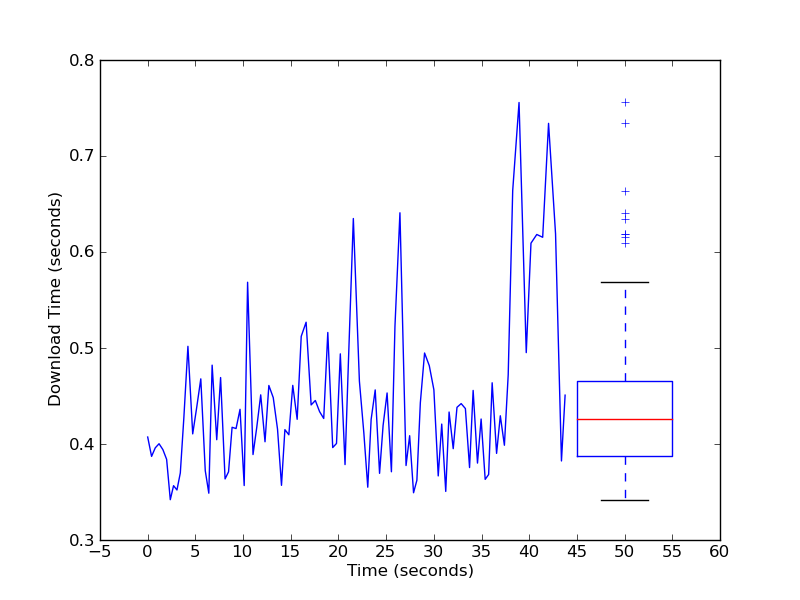
\includegraphics[width=11cm]{graphs/download-combined}

\section{Section Name}

$d_{trans}$ is the transmission delay. $d_{prop}$ is the propagation delay.

\begin{align*}
d &= d_{trans} + d_{prop}\\
  &= (1000*8)/1000000 + 0.05\\
  &= 0.058
\end{align*}

\end{document}
